% This is the Capstone paper draft 2 TeX document
% Composed 5/16/2018
% LLNCS macro package for Springer Computer Science proceedings;
% Version 2.20 of 2017/10/04
%
\documentclass{llncs}
%
\usepackage{graphicx}
% Used for displaying the figures. If possible, figure files should
% be included in EPS format.
%
% If you use the hyperref package, please uncomment the following line
% to display URLs in blue roman font according to Springer's eBook style:
% \renewcommand\UrlFont{\color{blue}\rmfamily}

\begin{document}
%
\title{A Geovisual Framework for Data Exploration in Government Open Data Using NIBRS (National Incident-based Reporting System) for Law Enforcement Agencies}
%
%\titlerunning{Abbreviated paper title}
% If the paper title is too long for the running head, you can set
% an abbreviated paper title here
%
\author{Michael Crowder\inst{1}\and
Lauren Darr\inst{1}\and
Gerardo Garza\inst{1}\and
Brent Allen\inst{1}}

%\authorrunning{M. Crowder et al.}
% First names are abbreviated in the running head.
% If there are more than two authors, 'et al.' is used.
%
\institute{Southern Methodist University Master of Science Data Science Program \and
Dallas, Texas, United States of America}
%
\maketitle              % typeset the header of the contribution
%
\begin{abstract}
In this paper we present a framework for creating geographic visualizations of criminal incidents using open data and open-source software. The motivation for this framework is to provide law enforcement agencies (LEAs) and interested citizens an affordable and relatively easy way to start analyzing geospatial data. The National Incident Based Reporting System (NIBRS) is a national standard for LEA incident reporting going into effect for all 18,000 U.S. LEAs in 2021. This project uses the Dallas Police Department'��s publicly available, NIBRS-style, incident data to develop a geovisual analysis method.    

\keywords{NIBRS  \and Visualization \and Cartography.}
\end{abstract}
%
%
%
\section{Introduction}
Open data is data that is freely available for use and redistribution by any individual without copyright restrictions\footnote{http://opendatahandbook.org/guide/en/what-is-open-data/} . Government agencies around the world are releasing government data in order to promote transparency, civic engagement, research and new services that benefit communities [1]. In the United States (U.S.), the Federal Bureau of Investigation (FBI) has used the Uniform Crime Reporting (UCR) program to promote transparency and generate reliable crime statistics for the U.S. since 1930\footnote{https://ucr.fbi.gov/}. The current UCR standard for LEAs is to report individual incidents via the National Incident Based Reporting System (NIBRS). As more LEAs conform to NIBRS, there is an increasing body of standardized incident reports available to LEAs and the public. Incident based crime reports are raw in format, not aggregated like the former UCR program reports. This format provides flexibility for exploring crime data.
\par The resources available to U.S. LEAs for crime data analysis are wide ranging. There are approximately 18,000 U.S. law enforcement agencies across federal, state, county, and local jurisdictions [2]. These agencies range in department size from 1-30,000 officers with the majority of agencies having 10 or fewer officers [2]. Furthermore, the fragmented nature of U.S. law enforcement as a collection of independent agencies makes the adoption of data handling practices disparate. This paper provides an introductory framework for geovisualization that can be affordably adopted by LEAs and engaged citizens interested in exploring geographical trends in police incidents. 
\par (Main results)
\par (Main Conclusions)
\par First, this paper explores the history of open data and the importance of open data to promoting the use of data analytics in new domains such as public safety. For the novice LEA or citizen data analyst this paper explains the critical process of exploratory data analysis (EDA). Then, the value of geographic visualizations is discussed in the context of the birth of computing and modern crime analytics. 
\par This paper moves on to describe the open source, NIBRS compliant, incident data of the Dallas Police Department used to build a framework for geovisualization. The methods section breaks down the major steps that should be taken to generate a reliable police incident map. Beyond the essential components of the framework, this paper lends examples of specific open source software and code that can be reused by novice crime analysts.

\section{History of open data}
The open data movement came on the heels of Internet globalization and is still developing rapidly [1]. In 2007 prominent academics and open data champions met to outline the guiding principles of open public data\footnote{http://parisinnovationreview.com/articles-en/a-brief-history-of-open-data}. In 2013, the U.S. government formally recognized open public data as a valuable national resource in a memorandum to the heads of executive departments and agencies titled “M-13-13 Open Data Policy-Managing Information as an Asset” [3]. The motivation behind the memo was to make information resources accessible, discoverable and usable by the public [3]. As one of the key pillars defined in the memo, accessibility suggests that open data must be made available in convenient, modifiable and open formats. These formats must be machine-readable and should be made available to the widest range of users for the widest range of purposes [3]. The larger goal of open data is to promote transparency in democratic governments, citizen participation, and drive innovation that can ultimately generate economic value\footnote{http://opendatahandbook.org/guide/en/why-open-data/} .
\par This project focuses on open data generated by the NIBRS set forth by the FBI UCR Program in partnership with the Bureau of Justice Statistics (BJS) in 1989. The NIBRS succeeded the Summary Reporting System (SRS) which provided aggregate statistics from law enforcement agencies with only one crime recorded per-incident regardless of the number of crimes that occurred\footnote{https://ucr.fbi.gov/nibrs/nibrs-user-manual}. NIBRS provides uncombined incident information that is more easily usable by interested parties. However, NIBRS has been slowly adopted by law enforcement agencies on a voluntary basis until now. Recently, the FBI set forth a NIBRS compliancy deadline of 2021 for all law enforcement agencies in the U.S. Former FBI director, James Comey, emphasized the importance of conforming to NIBRS in a 2015 speech to the International Association of Chiefs of Police (IACP): “NIBRS is a way in which we can collect data that will identify patterns, trends, and help us prevent crime and have thoughtful, informed conversations at the national level”\footnote{www.fbi.gov/audio-repository/news-speeches-comey-at-2015-iacp-conference.mp3/view} .

\section{What is exploratory data analysis?}
Exploratory data analysis (EDA) is a collection of tools and approaches used to understand data structure and gain general insight into a data set [4]. EDA is useful for testing statistical assumptions and generating new hypotheses and patterns [4]. In the 1970s, statistician John W. Tukey formalized the term EDA and emphasized the need to use exploratory methods such as visualization ‘to force us to notice what we never expected to see’ [5]. Tukey emphasized that exploratory methods were not simply descriptive statistics but crucial to accurately applying formal statistical tests [5].
\par EDA is a major component of developing a geovisual framework for NIBRS incident data. Before incident data can be mapped to a geographic plane, the data must be explored for accuracy, anomalies, and general understanding of the variables. EDA goes hand in hand with data cleaning or pre-processing. Section 4.3 ‘Data Pre-Processing’ details steps taken to explore and clean the example incident data. However, EDA is not limited to the steps taken in this project. It is important to remember that EDA and data cleaning are flexible and iterative processes highly dependent on the data set in use.
\par For users of a geovisualization it is likely that they are unfamiliar with the exact nature of the data. This type of situation calls for flexible geovisualizations that can be adapted by the user[17]. The presentation of a cartographic communication can include both the transfer of an already known message and could also bring new insights from the viewer that was not known when put together by the presenter of the cartographic communication[17]. 
\par Geovisuilization can be designed communicate to a wide audience and easily understood. Methods should look at questions like "What is?", "Where is?" and "What belongs together?". For example two seperate sets of information put on a table might not provide a lot of information, but if displayed spatial a user could start to define a relationship. Interactive geovisualizations allow users explore different parameters such as time, groups, and location, or philosophical perspective of a problem[18].

\section{Geographic visualization}
In 1962 Richard Hamming stated “The purpose of computing is insight, not numbers” [6]. Today, computing insight is often associated with the production of visualizations. Visualization in scientific computing was first described by a paper sponsored by the National Science Foundation in 1987. This paper described potential gain in productivity and breakthroughs in the American scientific and engineering communities with the increasing improvement of computer visualizations [7]. The main goal of visualization is to see the unseen by interpreting the data fed into a computer. The value of visualization in the scientific processes is manifold. Visualizations provide a way to generate new hypotheses through the EDA process. And, visualizations are commonly used as deliverables for describing the outcome of scientific investigation [8].
\par The use of data visualizations to improve scientific and technical reporting is not without challenges. One challenge in modern visualization is the use of large data sets. Wang et al. describes a few reasons why visualizing large data can become burdensome. First, visual noise is the phenomenon where too many data points are highly similar and cannot be graphically separated. One method of combatting visual noise is the reduction of data, but this generates the problem of information loss. Also, large image perception is confined by the limited aspect ratios of viewing devices as well as the perception limitations of humans. Unsurprisingly, data intensive visualizations may carry high performance requirements that are costly [9].
\par The general benefits and challenges of data visualizations are certainly applicable to geo-visualization. Maps have been in use for thousands of years, maps with data have been in use for almost as long. With the rapid rise of new data sources comes the challenge of how we extract useful information. Do authors of visualizations use the original data set or combine other datasets linked by say zip codes, or census tracks to make them more useful to the user? [10]. The classic definition of a map is that of a plot of land scaled down on a flat medium that represents part of the Earth’s surface. The rise of information technology and scientific computing have given rise to geographic information systems (GIS). A typical GIS software will have the ability to layer information on top of a map in order to tell a story with a dynamic map that a user can explore. 
\par There are many software types that exist for geospatial analysis. There are large commercial GIS packages like ArcView, ArcGis and ERSI. While the commercial GIS packages have served as industry standards for some years, open source GIS options are increasing. For example, open source software environments Python and R have GIS libraries such as Plotly, GeoPandas, and Leaflet that enable the creation of robust, interactive geospatial visualizations for free.

\section{Crime analytics}
It is unsurprising that news media coverage of crime data analytics has a tendency to focus on the most ground breaking and intriguing innovations of the moment. A 2016 Science Magazine article detailed the use of advanced predictive software by agencies looking both to predict where crimes will happen and the actual individuals who may commit or become victims of crimes [11]. For example, PredPol is proprietary software that uses algorithms to predict where crimes are likely to happen during a shift [11]. While forecasting crimes is a highly pertinent application of incident data, it is not a cure-all for understanding and effectively using crime data.
\par In 2015, the Police Data Initiative (PDI) was launched per recommendation of President Obama’s Task Force on 21st Century Policing\footnote{https://www.data.gov/safety/launching-the-police-data-initiative/}. The PDI is a collective network of law enforcement agencies, researchers, and technologists already developing and delivering best practices for collecting and publishing public datasets as well as utilizing data and technology for the improvement of policing and community relations. As of March, 2018, there are 130 contributing agencies and over 330 available data sets through the PDI website. The PDI demonstrates and embraces the diversity of law enforcement agencies’ needs and resources with both large and small department participants.


\section{Data}
\subsection{Data source}
Data was sourced from the Dallas Open Data website hosted by Socrata in order to provide an illustration of the process of using open source NIBRS compliant incident data\footnote{https://www.dallasopendata.com/}. This website is designed to provide transparency to citizens and developers with a variety of data sets that pertain to city governance, services, and culture. The NIBRS based data set of interest on Dallas Open Data is titled Police Incidents. The Police Incidents data set is provided by the Dallas Police Department and is updated daily with incident reports dating back to June 1, 2014.
\par As of May, 2018, there are approximately 357,000 incident entries and there are 103 incident attributes. The complete list of incident attributes is found in the appendix. Some important features of an individual incident report include the unique identifier, ‘Incident Number w/Year’, the location details of the incident, the descriptive details of the complainant, the reporting officer details, and the details of the type of incident that occurred.

\subsection{Accessing data}
The Police Incidents data set was accessed using the Socrata application programming interface (API) and R (version) programming language within the R-Studio (version) programming environment. 
**Include more information about how the API works, the documentation from Socrata and how the R Socrata library was used to access the data and store it into a df. Every time the code is run the df is updated with whatever new entries have been added to the data set.

\subsection{Pre-processing data}
Data pre-processing, or data cleansing, is the important step of determining what kind and how many inaccuracies are present in a data set. It is safe to assume that most data sets have inaccuracies. Examples of potential problems a data set may include: missing values, incorrect attribute data types, misspellings, incorrectly entered data, duplicate entries, and more (CITE some info about data cleaning process).

\section{Methods}
\subsection{Incident type: burglary}
There is a wide variety of incident types recorded every day by police departments everywhere. In order to effectively visually explore crime incidents, it is important to focus in on specific types of incidents. 
\par Cartographic interaction can be defined by the interaction between a human and map that is driven by a computing device [12]. We present 3 different types of interactive maps: Dot Map, Heat Map and Cluster Map.
\begin{figure}
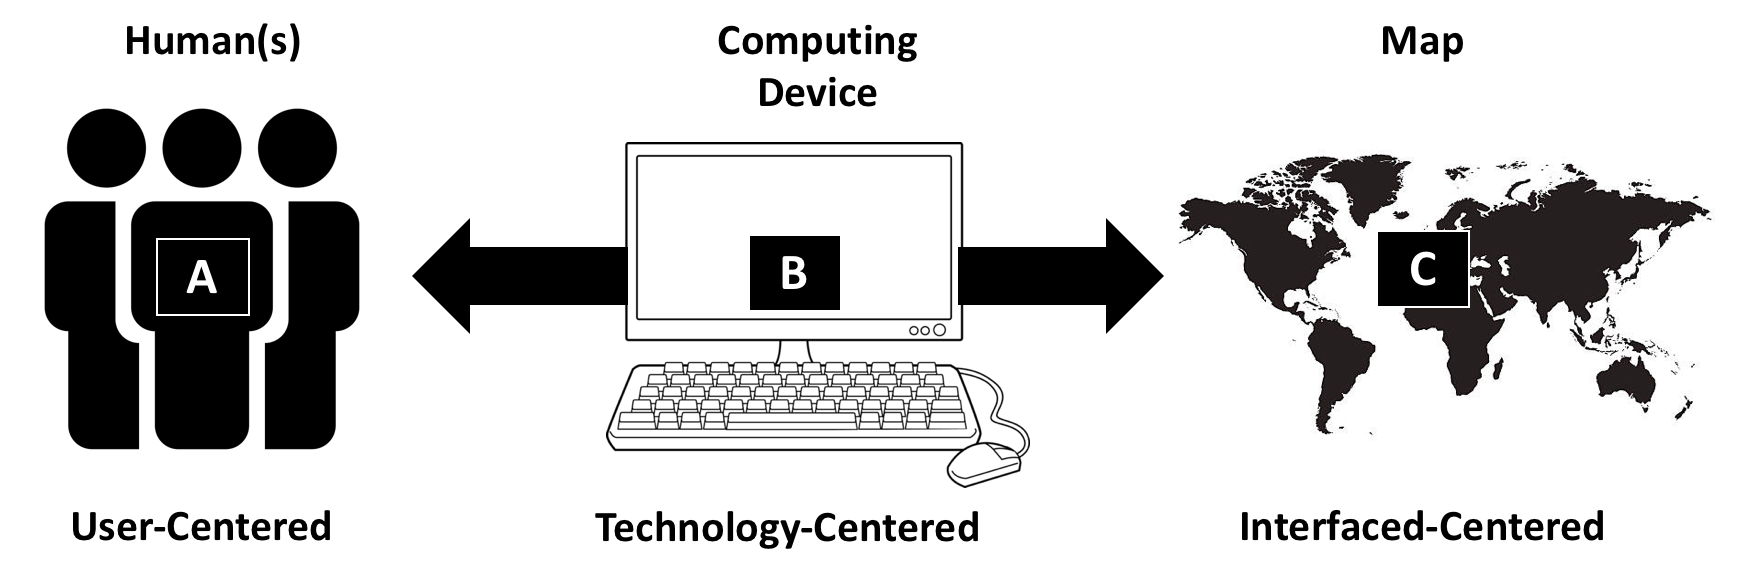
\includegraphics[width=\textwidth]{interactiveMapProcess}
\caption{Figure 1: Pieces of digital cartographic interaction. The figure represents the dialog between a human (A) a computing device (B) and a map (C). Figure reproduced from Roth [12].} \label{fig1}
\end{figure}
\par The method of interactive cartography was used to give the novice user the ability to engage in their own knowledge construction of what the mapmaker display of the event, or events.
\par Maps were created with an open source Java Script (JS) library for interactive maps called Leaflet (www.leafletjs.com). The API is offered in open source languages like R, and Python. Our maps were designed with the Leaflet R library. Leaflet’s products are also used in professional GIS programs like ARC GIS and ESRI.
\subsection{Dot Map}
\par A dot map shows the geographic distribution of an event or events through the placement of a dot to a single event, or a cluster of events [13]. For this paper we mapped each dot to a latitude and longitude coordinate and presented each incident as single event. The selection of a dot size can be an intuitive or processed approached [13]. The framework dot map is not based on a processed approached. The dot map that is presented in figure x is an interactive map or known in cartography as a cartographic interaction. This presented a decision about the radius of the dot. The dots on a dot map when not zoomed are large and scale to smaller dots upon zoom. At zoom it would approximate the locations very well. At the initialization of the map the user may not be able to engage in their own knowledge construction.
\begin{figure}
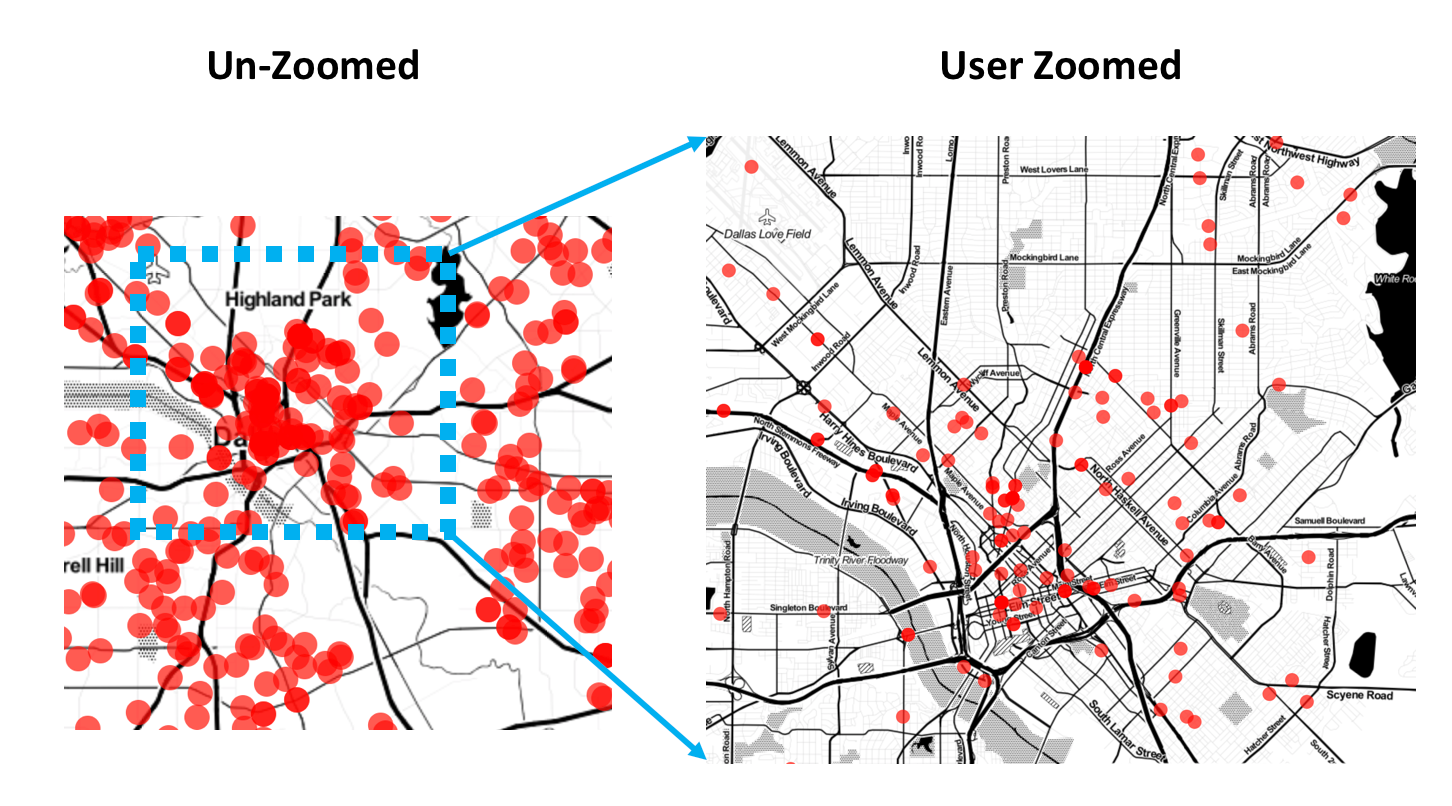
\includegraphics[width=\textwidth]{dotMapDrawbacks.png}
\caption{Figure 2: Shows the drawback of interactive dot maps when scale is not adjusted on the zoom.} \label{fig2}
\end{figure}
\subsection{Heat Map}
\par The second method of mapping we present is the heat map. Heatmaps are widely used in displaying levels, or differences when a distribution of point data is close together[15]. Density analysis is utilized when analyzing heatmaps. Specifically kernel density is used in our heat map by assigning the highest value to the closes crime and values are lowered as distanced becomes greater. The function K is conveyed in the equation
\[ f(x,y) = \frac{1}{nh^d}\sum_{i=1}^{n} K\frac{x-x_i}{h} \]
where n = total number of points, h = bandwidth to determine the amount of smoothing, K = kernel function, d = data dimensionality, x = location of estimated point, and x {i} = the location of known point i.
Colors in red represent are denser areas of activity. As the distance in clustered points increases the gradient becomes orange, yellow, green and then a greenish blue. 
\begin{figure}
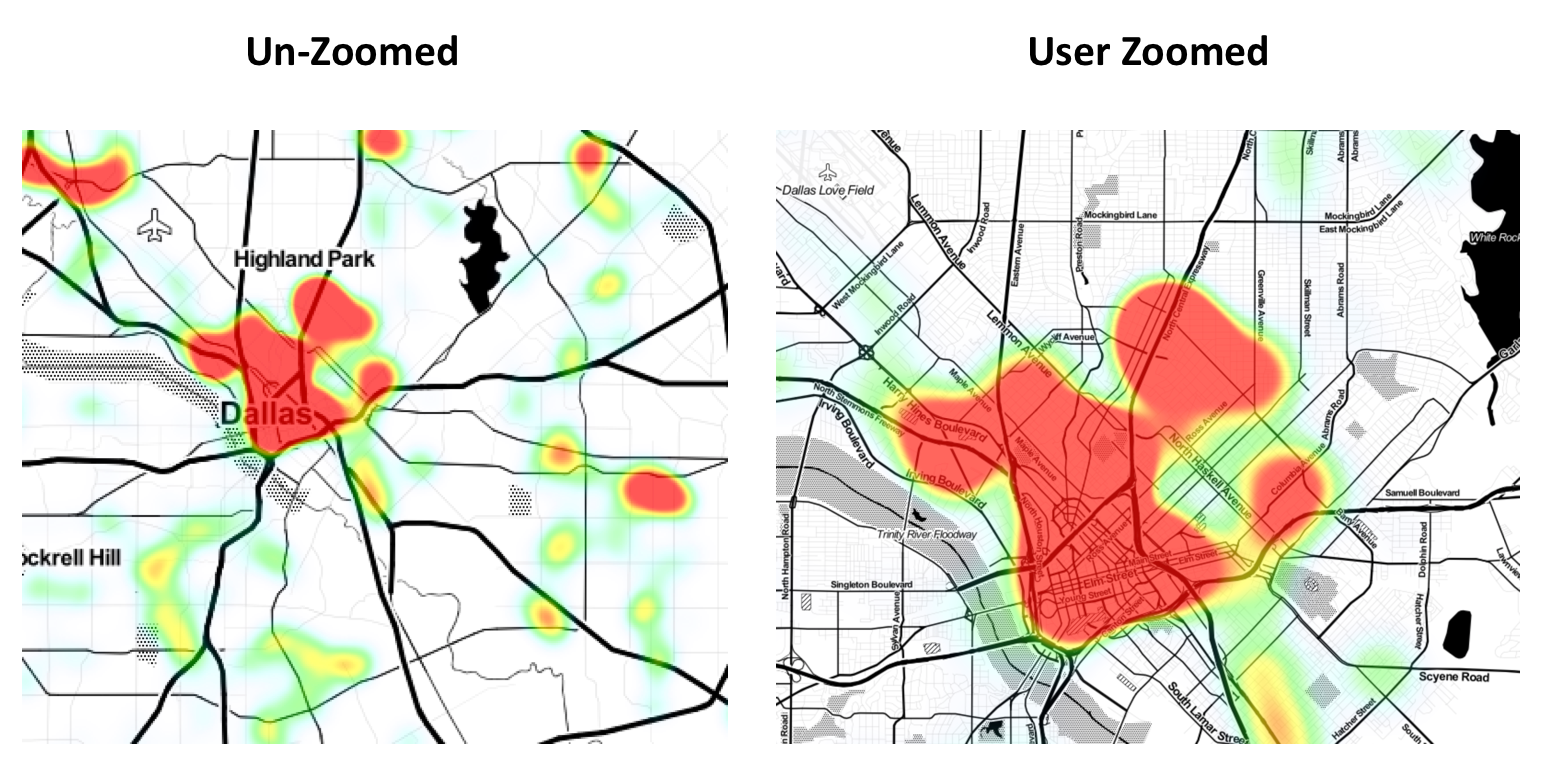
\includegraphics[width=\textwidth]{heatMapExample.png}
\caption{Figure 3: Shows heat map un-zoomed and zoomed} \label{fig3}
\end{figure}
\par Heat maps do come with some drawbacks. They can be difficult to compare objectively. Classification systems cannot be adapted for most software packages. Heatmaps can also be problematic because they may not be the right choice for the detection of extreme values[16].

\subsection{Cluster Map}
\subsection{Burglary: mapped by zip code}
\subsection{Burglary: mapped by zip code and year}

\section{Ethical considerations}
The dataset we use in this paper contains the names and addresses of complainants of the burglaries displayed in this research. We did not map out the addresses of the complainants of the burglaries, there was no reason to do so. The practice of including the name and address of the complainant is actually very common in public safety open datasets. Unwarranted publication of personal addresses could pose a threat to those that report crimes. There also inlies the possibility of businesses scraping the data of complainants to target advertisements and products in what could be a sensitive time for the complainant. 
\par The “Incident Address” in our data is the address where an incident occurred. There exist many possible ways in which data can be displayed on maps. Heat maps present opportunities to adjust density in order to magnify the visualization of incident location. This could cause the potential for an area to appear to have more activity than it actually does. If a user of the geovisual tool is looking at say crime in an area they are considering purchasing a house, or a user is looking for a place to place a business the density on the heat map could turn that user away from an otherwise safe area.
\indent Those preparing geovisualization for novice users should take into account potential considerations on how the visualization could affect an individual party, or a community as a whole. A famous case of geovisualization in journalism occurred in 2012 just months after the Sandy Hook Elementary shooting. The publication published three online maps that contained a two-county area with the names and addresses of those that were permit holders. 
\par Some ground-rules, or guidelines to consider when preparing a geovisualization for novice users would be to research data journalism guidelines. Craig, Ketterer, and Yousuf, in their paper “To Post or Not to Post: Online Discussion of Gun Permit Mapping and the Development of Ethical Standards in Data Journalism provides some recommended frames when considering publishing information that could raise ethical questions. The first is freedom verus responsibility and journalistic purpose, which purposes that data should not be posted only because its already in a public dataset. The second frame is privacy and verification, to attempt to measure the risks to a person’s private life. Thirdly are consequences to the individual if the information is wrong. Finally, what alternatives are available, such as showing trends or joining with other data to tell the same story [14].
\section{Conclusion}

%
% ---- Bibliography ----
% Bibliography has not been updated as of 4/25/18 
% BibTeX users should specify bibliography style 'splncs04'.
% References will then be sorted and formatted in the correct style.
% \bibliographystyle{splncs04}
% \bibliography{mybibliography}
%
\begin{thebibliography}{8}
\bibitem{ref_article1}
Jaakola, A., Kekkonen, H., Lahti, T., and Manninen, A.: Open data, open cities: Experiences from the Helsinki Metropolitan Area. Stat J IAOS (1), 117--122 (2016)

\bibitem{ref_article2}
Banks, D., HIckman, M., Kyckelhan, T.: National Sources of Law Enforcement Employment Data. U.S. Department of Justice: Office of Justice Programs, Bureau of Justice Statistics (2016)

\bibitem{ref_article3}
Burwell, S., VanRoekel, S., Park, T., and Mancini, D.: M-13-13: Open Data Policy-Managing Information as an Asset. Executive Office of the President, Office of Management and Budget, Washington DC (2013)

\bibitem{ref_article4}
Jebb, A.T., Parrigon, S., and Woo, S.E.: Exploratory data analysis as a foundation of inductive research. HRMR 27 (2017), 265-276

\bibitem{ref_article5}
Tukey, J.W.: Exploratory Data Analysis. Addison-Wesley Pub. Co. Reading, MS (1977)

\bibitem{ref_article6}
Hamming, R.: Numerical Methods for Scientists and Engineers. McGraw-Hill, New York (1962)

\bibitem{ref_article7}
McComick, B.H. et al.: Visualization in Scientific Computing. Computer Graphics ACM SIGGRAPH21, New York 6(1987) 1-81

\bibitem{ref_article8}
Ma, X., et al.: Using visual Exploratory Data Analysis to Facilitate Collaboration and Hypothesis Generation in Cross-Disciplinary Research. ISPRS Int. J. Geo-Inf, 6(11) (2017) 368+

\bibitem{ref_article9}
Wang, L., Wang, G., and Alexander, C.A.: Big Data and Visualization: Methods, Challenges, and Technology Progress. Digital Technologies 1(1) (2015) 33-38

\bibitem{ref_article10}
J.H. Kwakkel, et al.: Visualizing geo-spatial data in science, technology, and innovation. Technol. Forecast. Soc. Change 81(C) (2014) 67-81

\bibitem{ref_article11}
Hvistendahl, M.: Crime Forecasters: Police are turning to big data to stop crime before it happens. But is predictive policing biased-and does it work?. Science, 353: 6307 (2016) 1484-1487

\bibitem{ref_article12}
Roth, R.E.: Interactive Maps: What we know and what we need to know. JOSIS, 6 (2013) 59-115

\bibitem{ref_article13}
Craig, D., Ketterer, S. and Yousuf, M.: To Post or Not to Post: Online Discussion of Gun Permit Mapping and the Development of Ethical Standards in Data Journalism, J. Mass Commun. Q., 94(1) (2017) 168-188

\bibitem{ref_article14}
Kimerling, A.J.: Dotting the Dot Map. Cartogr. Geogr. Inf. Sc., 36(2) (2016) 165-182

\bibitem{ref_article15}
Hong, Ilyoung: What Is So "Hot" in Heatmap? Qualitative Code Cluster Analysis with Foursquare Venue, The International Journal for Geographic Information and Geovisualization 

\bibitem{ref_article16}
Study of the attentive behavior of novice and expert map users using eye tracking, Cartography and Geographic Information Science 

\bibitem{ref_article17}
Maceachern, A.,Kraak, J. Exploratory Cartographic Visualization: Advancing the Agenda, Computers and Geosciences (1997)
\end{thebibliography}

\subsubsection{Acknowledgments} 

\begin{figure}
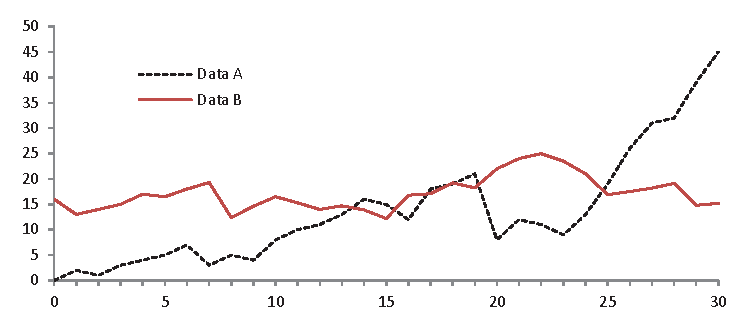
\includegraphics[width=\textwidth]{fig1.eps}
\caption{A figure caption is always placed below the illustration.
Please note that short captions are centered, while long ones are
justified by the macro package automatically.} \label{fig1}
\end{figure}

\end{document}
